\appendix
\chapter{Appendix A: Reconfigurable moderator in TAP core}
\label{appex:geometries}

\renewcommand{\thetable}{A.\arabic{table}}
\setcounter{table}{0}
\renewcommand{\thefigure}{A.\arabic{figure}}
\setcounter{figure}{0}
%%%%%%%%%%%%%%%%%%%%%%%%%%%%%%%%%%%%%%%%
\begin{table}[h!]
	\caption{Geometric details for the full-core 3D model of the \gls{TAP} 
	with various moderator rod assemblies configurations. }
	\begin{tabularx}{\textwidth}{ X X X X}
		\hline
		Case & Number of ZrH$_{1.66}$ & \gls{SVF} & Moderator-to-\\ 
		     & rods in the quarter core   &          & fuel ratio			\\ 
		     \hline
		1 (\gls{BOL}) &  347          & 0.917204 & 0.09027              \\
		2    &        406             & 0.903126 & 0.10727              \\
		3    &        427             & 0.898115 & 0.11344              \\
		4    &        505             & 0.879503 & 0.13700              \\
		5    &        576             & 0.862563 & 0.15933 		        \\
		6    &        633             & 0.848962 & 0.17791      	    \\
		7    &		  681			  & 0.837509 & 0.19402	            \\
		8    &        840             & 0.799571 & 0.25067              \\
		9    &        880             & 0.790026 & 0.26578              \\
		10   &        900             & 0.785254 & 0.27347              \\
		11   &        988             & 0.764257 & 0.30846 		        \\
		12   &        1126	          & 0.731329 & 0.36737      	    \\
		13   &		  1338	    	  & 0.680744 & 0.46898	            \\
		14   &		  1498			  & 0.642567 & 0.55626	            \\
		15 (\gls{EOL})& 1668          & 0.602004 & 0.66112              \\
		\hline
	\end{tabularx}
	\label{tab:tap_adjustable_core}
\end{table}
%%%%%%%%%%%%%%%%%%%%%%%%%%%%%%%%%%%%%%%%%%%%%%%%%%%%%%%%%%%%%%%%%%%%%%%%%%%%%%%
\newpage
\begin{figure}[htp!] % replace 't' with 'b' to 
	\centering
	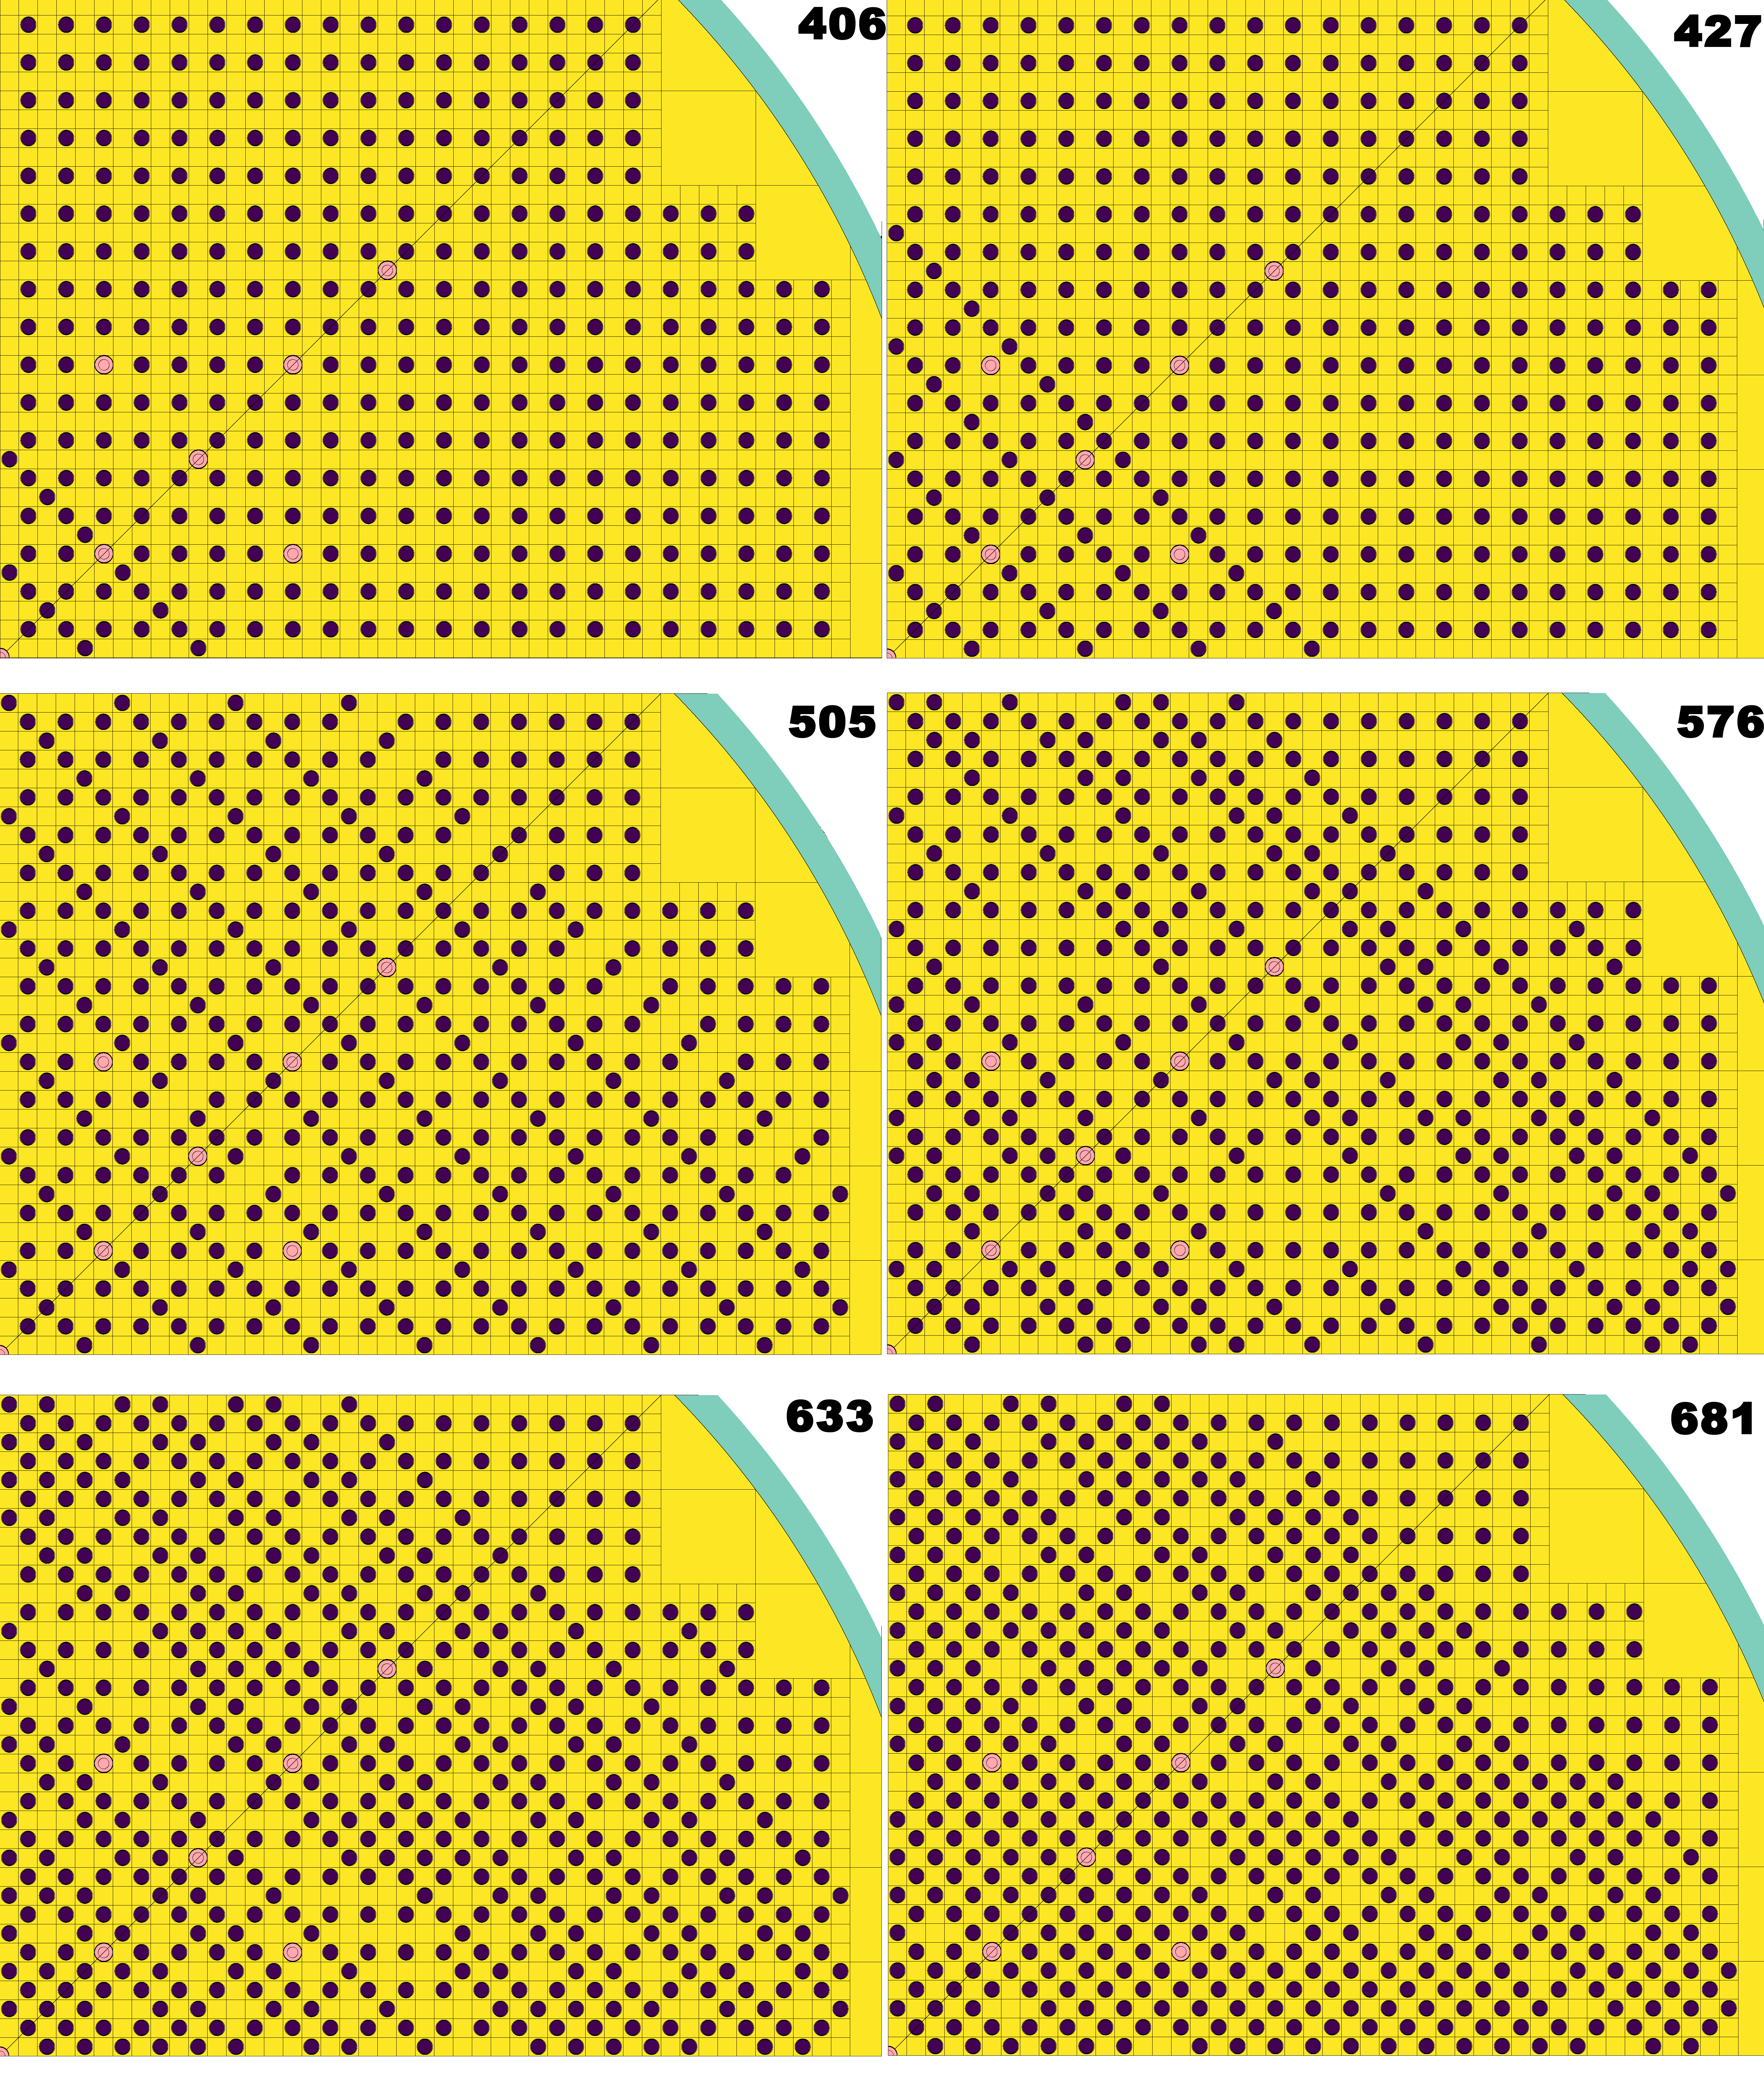
\includegraphics[width=\textwidth]{appex/tap_406-681.png}
	\caption{An $XY$ section of the \gls{TAP} model at horizontal midplane for 
	the first six years of operation (excluding startup moderator rods 
	configuration) with the \gls{SVF} between 0.91 and 0.84. The number in the 
	top-right corner of each figure indicates the number of moderator rods in 
	the case.}
	\label{fig:tap-406-681}
\end{figure}

\newpage
\begin{figure}[htp!] % replace 't' with 'b' to 
	\centering
	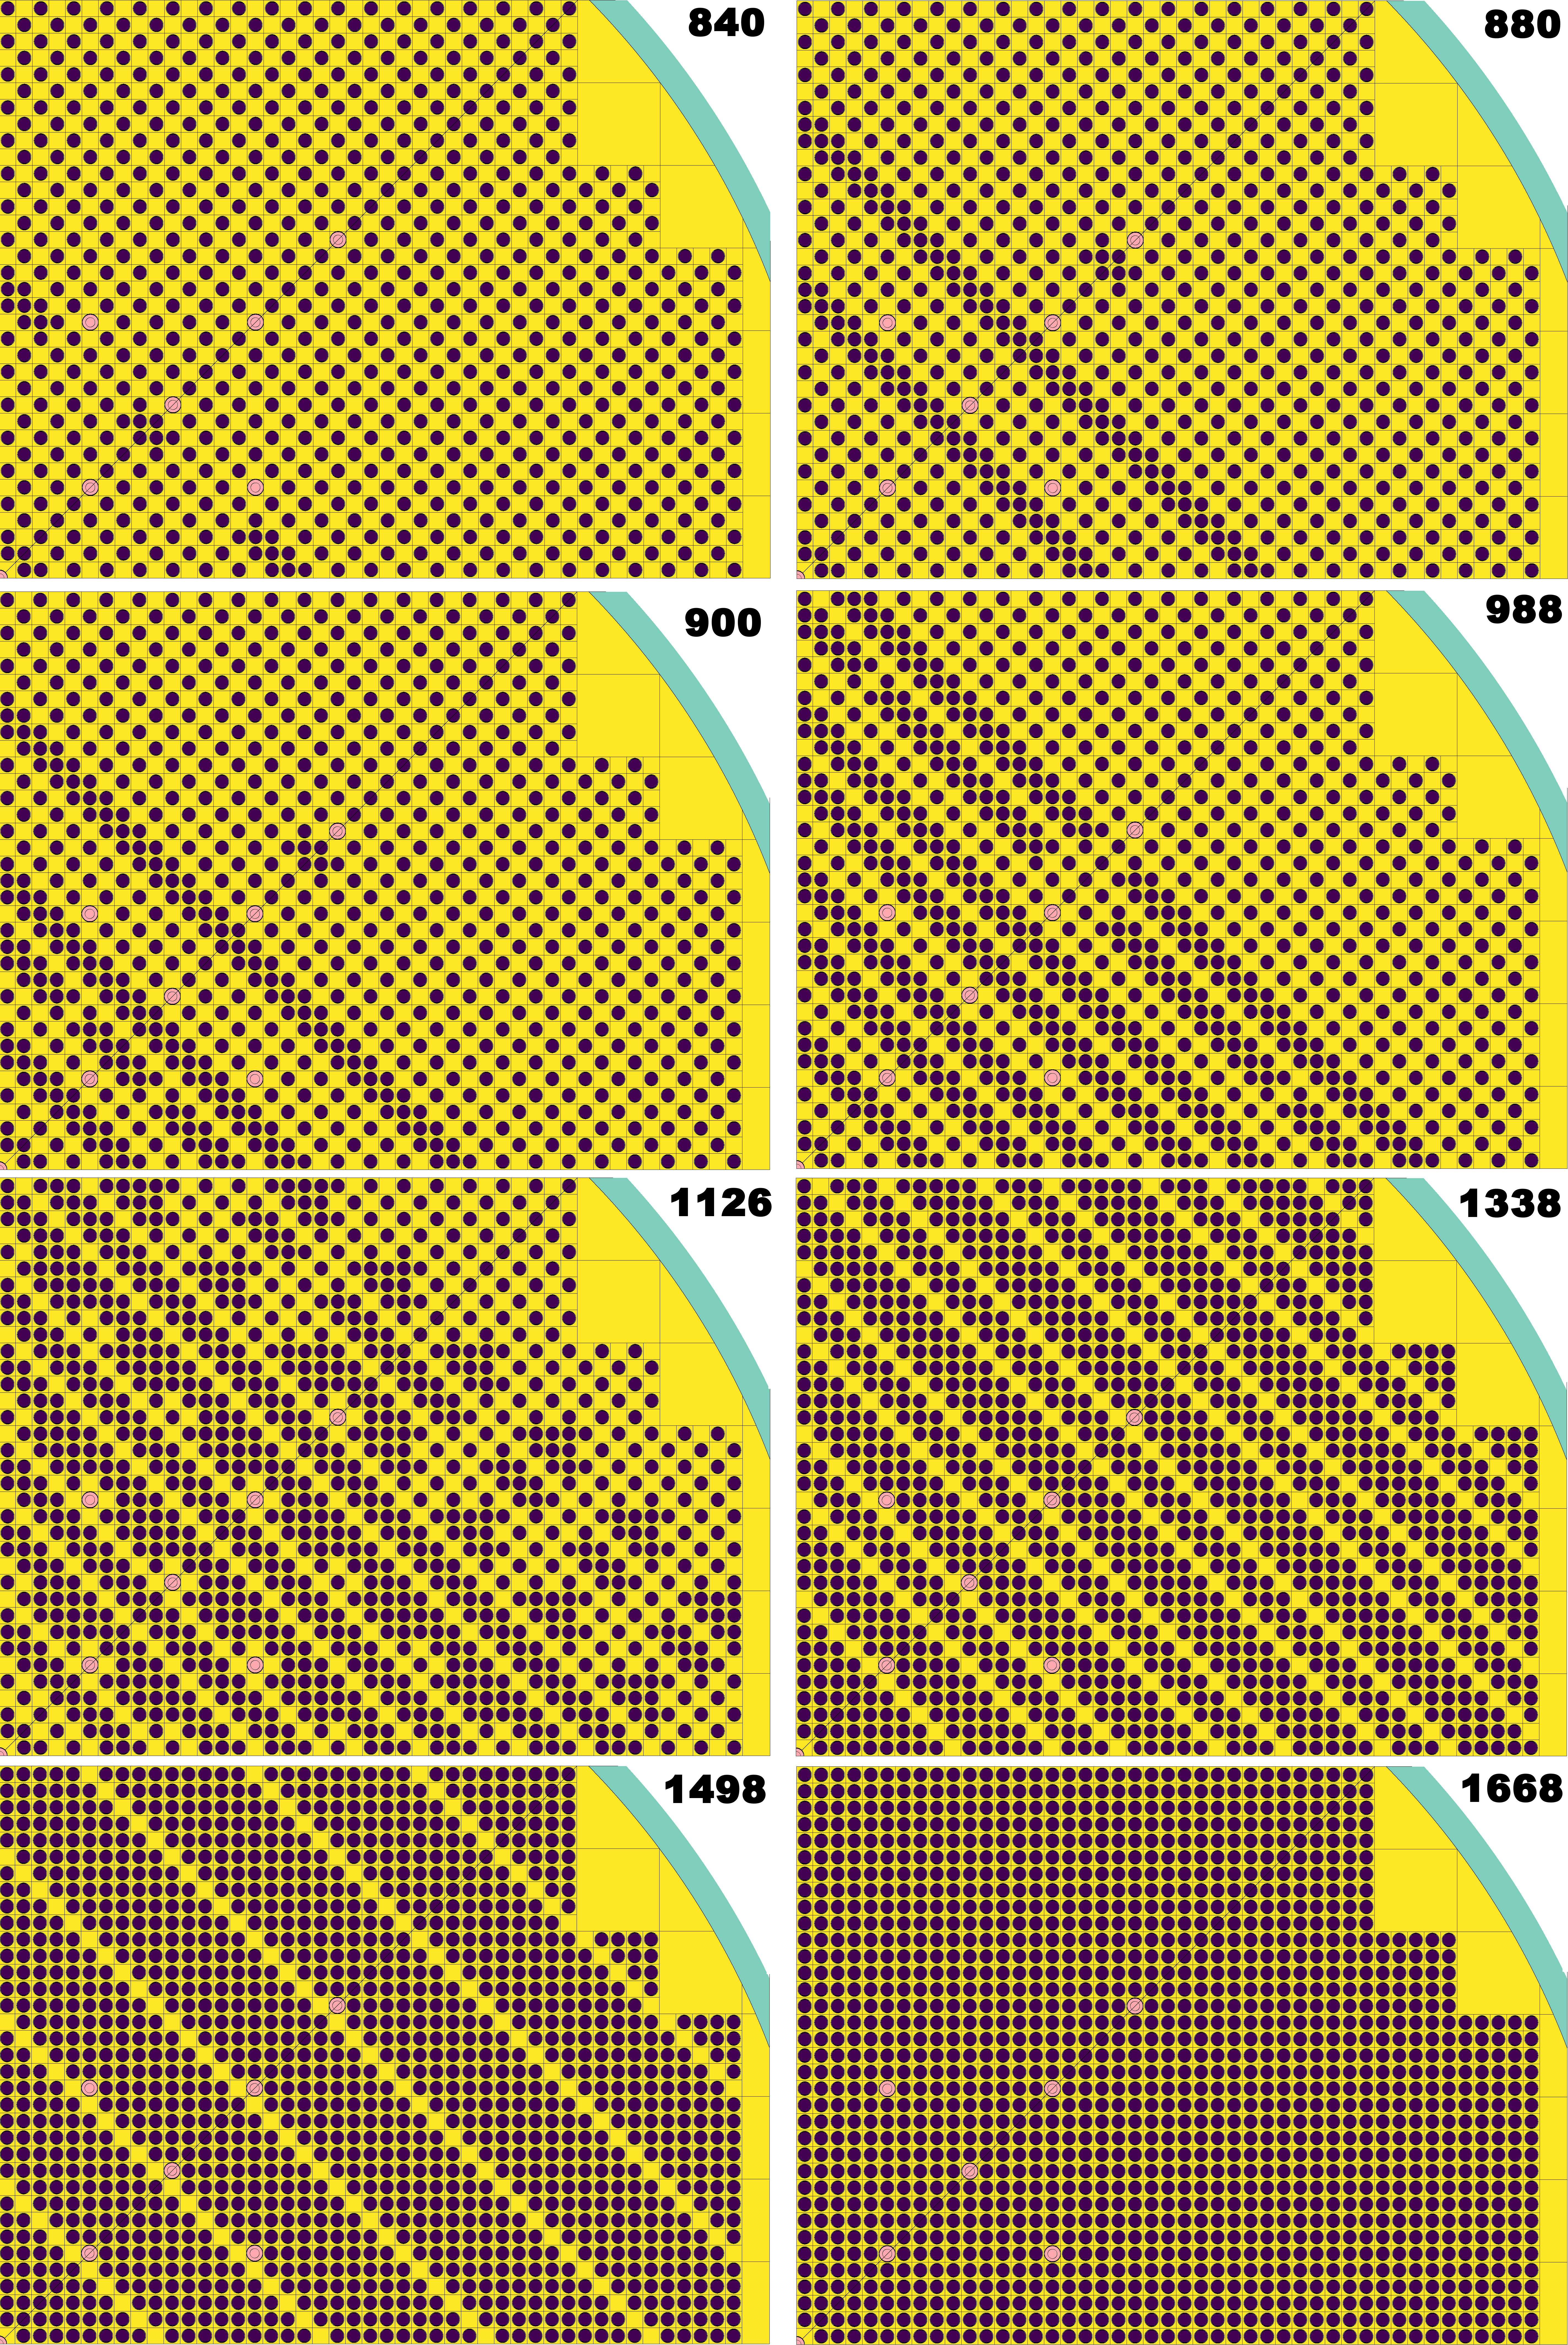
\includegraphics[width=0.9\textwidth]{appex/tap_840-1668.png}
			\vspace{-3mm}
	\caption{An $XY$ section of the \gls{TAP} model at horizontal midplane the 
	\gls{SVF} between 0.8 and 0.6. The number in the top-right corner of 
	each figure indicates the number of moderator rods in the case.}
	\label{fig:tap-840-1668}
\end{figure}

